
\chapter{Motivation}
\label{cha:motivation}
In this chapter, we describe the motivations behind adding copatterns to
Idris. We find that copatterns can be a means of recovering from an unfortunate
loss of subject reduction. However, copatterns might not be the universal tool
for coinductive reasoning. Additionally, we motivate the addition of an
inference system for guarded recursion.

\section{Recovering Subject Reduction}
\label{sec:recov-subj-reduct}
%#########
% Hvorfor mistes subject reduction ved dependent pattern matching på codata?
% Mister Idris subject reduction?
% Modeksempel (helst implementeret i Idris)
% Hvordan afhjælper copatterns problemet?

% Ny viden: Copatterns kan være et værktøj til at undgå at man mister subject reduction
%#########
Subject reduction is a property of a type system. Also called type preservation,
a type system has the property of subject reduction if evaluation of a
well-typed term does not cause its type to change\,\citep[Section~8.3.3]{Pierce:2002:TPL:509043}.
In some dependently typed programming languages with explicit coinductive types,
e.g. Coq and Idris, values of such types are given as (potentially) infinite
trees of constructors. Accordingly, they can be analysed with (dependent)
pattern matching. However, this leads to a loss of subject reduction. The
problem was first identified by Gim\'{e}nez\,\citep{Gimenez96uncalcul} for the
Calculus of (Co)Inductive constructions, but was later (in 2008) shown by Oury
to persist in both Coq and
Agda\,\citep{OuryCounterexampleCoq,OuryCounterexampleAgda}.

By implementing Oury's counterexample
(Figure~\ref{fig:ourys_counterexample_idris}), we have found that the problem
arises in Idris as well. Oury's counterexample unfolds as follows: Given a
coinductive type \texttt{A} with a single constructor \texttt{A} $\to$ \texttt{A}, which we may call
\texttt{In}, and an inhabitant \texttt{b} of \texttt{A} (of which there exists only one,
namely the fixed point of \texttt{In}), we can show that \texttt{b} is definitionally
equal to its own unfolding by exploiting dependent pattern matching. When
\texttt{b} is given as argument to \texttt{forceEq} in
Figure~\ref{fig:ourys_counterexample_idris}, \texttt{b} is reduced to \texttt{In
  (Delay (In (Delay a)))} by dependent pattern matching, such that \texttt{forceEq b}
reduces to \texttt{Refl}. These reductions ensure that the implementation of
\texttt{p} is well-typed. The problem arises when we attempt to replace the
right-hand side of \texttt{p} with \texttt{Refl}, which is the definition of
\texttt{forceEq b}. In this case, the Idris type checker rejects the program,
complaining that \texttt{b} cannot be unified with \texttt{In b}. Thus, the
evaluation of \texttt{forceEq b} changes the type of \texttt{Refl}, and subject
reduction is lost.

\begin{figure}
\begin{lstlisting}[mathescape]
codata A : Type where
  In : A $\to$ A

b : A
b = In b

force : A $\to$ A
force (In (Delay (In (Delay a)))) = In (Delay (In (Delay a)))

forceEq : (x : A) $\to$ x = force x
forceEq (In (Delay (In (Delay a)))) = Refl

p : b = In (In b)
p = forceEq b
\end{lstlisting}
  \caption{Oury's counterexample implemented in Idris, leading to a loss of
    subject reduction.}
\label{fig:ourys_counterexample_idris}
\end{figure}

Dependent pattern matching on coinductive data is problematic, but we cannot
simply disallow it, since we then lose the ability to write any interesting
programs involving coinductive data. This ability can be regained by introducing
copatterns. Instead of analysing coinductive data with dependent pattern
matching, we can choose to synthesize it using copatterns. In
Figure~\ref{fig:ourys_counterexample_copatterns}, we have translated Oury's
counterexample to an Idris implementation with copatterns, where we have
refrained from using dependent pattern matching. Using copatterns, we can still
define both \texttt{b} and \texttt{force}, but we cannot provide an
implementation for \texttt{p}, since the reduction behaviour from dependent
pattern matching is (virtually) unavailable. Hence, we have both regained
expressiveness and avoided this particular loss of subject reduction.

\begin{figure}[h]
\begin{lstlisting}[mathescape]
corecord A : Type where
  out : A $\to$ A

b : A
&out b = b

force : A $\to$ A
&out force a = out a
&out &out force a = out (out a)

forceEq : (x : A) $\to$ x = force x
forceEq a = $\uwave{\text{Refl}}$

p : b = out (out b)
p = $\uwave{\text{forceEq b}}$
\end{lstlisting}
  \caption{By using copatterns to synthesize coinductive data, we can both
    implement functions on coinductive data and preserve subject
    reduction. The underlined right-hand sides indicate type errors detected by
    the Idris type checker.}
\label{fig:ourys_counterexample_copatterns}
\end{figure}

In Agda, pattern matching on coinductive data is currently
disallowed\,\citep{Danielsson09}, providing the user with copatterns instead. By
implementing copatterns in Idris, we provide a stepping stone in the same
direction. However, this solution may seem to avoid the problem, rather than
solving it. As pointed out by McBride\,\citep{McBride:2009}, the underlying
problem is that we can have intensional equalities between coinductive values
which are merely bisimilar. To remedy the situation, he proposes that one could
have an observational propositional equality, which takes into account both
functional extensionality and bisimilarity for coinductive values. Also,
Altenkirch et al.\,\citep{Altenkirch:2007} proposes the adoption of an
observational type theory, which is essentially an intensional type theory where
one can have propsitional equalities up to observation, as opposed to
construction. But until these ideas are incorporated into a practical system,
avoiding the problem seems superior to ignoring it.


\section{The Use Case for Copatterns}
\label{sec:motivation_copatterns}
%############
% Pattern matching on data with top-level product structure vs. copatterns
% Mixed induction-coinduction, coinductive resumption monad
% Coinduction (definition og operationel intuition) (måske bisimilarity)

% Ny viden: Hvornår bør/kan jeg bruge copatterns?
%############
% Pattern matching has become a ubiquitous tool for analysing data in functional
% programming languages. In combination with inductive data types, pattern
% matching has evolved into such a widely applicable technique that many users may

% be willing to disregard its drawbacks. Consider the following implementation of
% a function which interleaves a filtered version of \texttt{xs} with \texttt{ys}:
% \begin{lstlisting}[mathescape]
% interleaveFilter : (a $\to$ Bool) $\to$ Stream a $\to$ Stream a $\to$ Stream a
% interleaveFilter p (x :: xs) (y :: ys) = 
% if p (head xs) then case xs of 
%                      xx :: xxs 
%    case (filter p xs) of
%      px :: _ => (px :: y :: (interleaveFilter p xs ys)
% \end{lstlisting}
% \begin{lstlisting}[mathescape]
% interleaveFilter : (a $\to$ Bool) $\to$ Stream a $\to$ Stream a $\to$ Stream a
% head       (interleaveFilter p xs ys)  = head (filter p xs)
% head (tail (interleaveFilter p xs ys)) = head ys
% tail (tail (interleaveFilter p xs ys)) = 
%                                interleaveFilter p (tail xs) (tail ys)

% mapNth : (a -> b) -> Nat -> Nat -> Stream a -> Stream b
% mapNth f (S n') m s = case s of
%                        x :: xs => x :: mapNth f n' xs
% mapNth f Z m s = case s of
%                   x :: xs => f x :: mapNth f m m xs

% \end{lstlisting}

%\subsection{Copatterns are Useful for Record Types}
% Recursive types!
\label{sec:prod-vs.-copr}
If we must disallow pattern matching on coinductive data to preserve subject
reduction, how much expressiveness can we recover by using copatterns? At
present, not as much as one might have hoped. Copatterns are well-suited for
working with data that has a top-level product structure. In the general sense
of recursive types, this means that copatterns can be readily used for types
which has a product-of-sums structure, i.e.
${\mu X.\,A\times B\times\cdots\times X}$ or
${\nu X.\,A\times B\times\cdots\times X}$, since a well-defined projection
exists for each $A,\,B,\,\cdots,\,X$. In Idris, this amounts exactly to the
types which can be defined as (co)inductive record types. Consider the
deterministic finite automaton defined in Figure~\ref{fig:state_machine}, which
accepts strings of binary numbers that contain an even number of zeros (a
graphical representation is given for reference in
Figure~\ref{fig:state_machine_graphical}). Inspired by
Jacobs\,\citep{JacobsCoalgebra}, we define a state as a type
${\mu S. (A\,\to\,S)\times Bool}$, where $A\,\to\,S$ is the transition function
(defined for each state) and $Bool$ indicates whether the state is a final
(i.e. accepting) state. Consequently, we can define each state (\texttt{SA} and
\texttt{SB} in Figure~\ref{fig:state_machine}) quite elegantly using copatterns.

\begin{figure}[h]
\begin{lstlisting}[mathescape]
data Binary = Zero | One

record State a where
  transitions : a $\to$ State a 
  isFinal     : Bool

mutual  
  SA : State Binary
  &transitions SA = ts
   where
     ts : Binary $\to$ State Binary
     ts Zero = SB
     ts One  = SA
  &isFinal     SA = True 
  
  SB : State Binary
  &transitions SB = ts
   where
     ts : Binary $\to$ State Binary
     ts Zero = SA 
     ts One  = SB
  &isFinal     SB = False

isAccepted : List Binary $\to$ Bool
isAccepted = isAccepted$'$ SA
  where
   isAccepted$'$ : State Binary $\to$ List Binary $\to$ Bool
   isAccepted$'$ s []        = isFinal s
   isAccepted$'$ s (b :: bs) = isAccepted$'$ ((transitions s) b) bs
\end{lstlisting}
  \caption{A finite state machine implemented using copatterns, identifying
    binary strings which contain an even amount of zeros.}
\label{fig:state_machine}
\end{figure}

\begin{figure}[h]
\centering
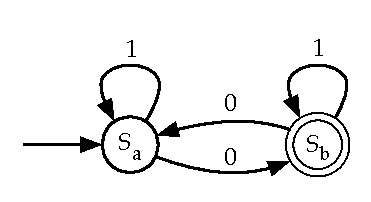
\includegraphics{figures/dfa}
\caption{A graphical representation of the automation defined in
  Figure~\ref{fig:state_machine}.}
\label{fig:state_machine_graphical}
\end{figure}

Unfortunately, copatterns are not very well-suited for types that have a top-level
sum-of-products structure, i.e. ${\mu X.\,A + B + \cdots + X}$ and
${\nu X.\,A + B + \cdots + X}$, because values of such types can take on
different forms in different contexts. In other words, the observable behaviour
depends on a further analysis, and the projections must therefore make
such an analysis possible. Consider the possibly infinite list encoded in
Figure~\ref{fig:colist}. Here, it is not possible to have a projection that
accesses the first element of a \texttt{CoList} directly, since it may be
empty. Instead, we can access an unfolding of the list, which may give either
answer.

\begin{figure}[h]
\begin{lstlisting}[mathescape]
corecord CoList a where
  unfold : Either (a, CoList a) ()

map : (a $\to$ b) $\to$ CoList a $\to$ CoList b 
&unfold map f xs = case (unfold xs) of
                      Left (x, xs) => Left (f x, map f xs)
                      Right () => Right ()
\end{lstlisting}
  \caption{A possibly infinite list type and a \texttt{map} function operating on it.}
  \label{fig:colist}
\end{figure}

The inherent uncertainty or ambiguity in types with sums-of-product structure
cannot be elegantly handled with copatterns. We can try to eliminate the need
for further analysis by tagging all values with an indicator of its state, as
shown with the modified CoList in Figure~\ref{fig:dependent_colist}. However, as
soon as the value of the tag is given indirectly, e.g. by reference to other values,
the type checker may become unable to reduce the tag to a canonical form, thereby
defeating its purpose.

\begin{figure}[h]
\begin{lstlisting}[mathescape]
corecord CoList a where
  isNil : Bool
  elem  : if isNil then () else (a, CoList a)

nil : CoList a
&isNil nil = True
&elem  nil = ()

cons : a $\to$ CoList a $\to$ CoList a
&isNil cons x xs = False
&elem  cons x xs = (x, xs)

toggle : Nat $\to$ Nat $\to$ CoList Nat
&isNil toggle n m = False
&elem toggle n m = (n, (cons m (toggle m n)))
\end{lstlisting}
\caption{A version of CoList defined with a boolean tag indicating whether
  additional elements of the list are available.}
\label{fig:dependent_colist}
\end{figure}

Since many useful techniques involve coinductive types which do not have a
straightforward product-of-sums structure, e.g. coinductive
resumptions\,\citep{Pirog2014273} and mixed
induction-coinduction\,\citep{Danielsson09mixinginduction}, \texttt{co}patterns
are therefore not necessarily a valuable tool for defining all kinds of
\texttt{co}inductive data. Instead, they provide elegant definitions when your data can be
clearly defined by its external properties, rather than by its internal
structure. Hence, we find copatterns at this stage to be universally \emph{applicable}, but not
universally \emph{useful}.


\section{Less Restrictive Productivity Checking} 
\label{sec:less-restr-prod}
% Hvorfor vil vi inferere guarded recursion?
%###########
% Dette afsnit har i princippet intet at gøre med copatterns!
% Referer til baggrund om syntactic guardedness
% Hvad kan guarded recursion som syntactic guardedness?
% Hvorfor er guarded recursion frygteligt at skrive / ikke brugervenligt?
% Bedre end syntactic guardedness + Bruger vil ikke skrive det => Inferer det


% Ny viden: Hvorfor vil vi gerne inferere guarded recursion?
%###########
Because the current productivity checker in Idris uses the syntactic
guardedness principle to prove productivity, users writing programs on
coinductive types must place all recursive calls directly under a call to a
coinductive constructor. This limitation means that we cannot have simple
definitions such as \texttt{toggle} from Figure~\ref{fig:dependent_colist}
proven total by the compiler. Using the technique of guarded recursion presented
in Section~\ref{sec:guarded-recursion} we are able to prove that toggle is
total, as shown in Figure~\ref{fig:toggle_guarded_recursion}. The proof is quite
involved, as it also requires us to define guarded recursive versions of
\texttt{cons} and \texttt{CoList} on which the original definition of
\texttt{toggle} depends. The coinductive \texttt{CoList} must be amended such
that the recursive reference in the \texttt{elem} projection is not be
immediately available.

\begin{figure}[h]
\begin{lstlisting}[mathescape]
corecord $_g$CoList a where
  isNil : Bool
  elem  : if isNil then () else (a, $\laterkappa$(CoList a))
  constructor CoCons

cons : $\forall\kappa.$ a $\to$ $_g$CoList a $\to$ $_g$CoList a
cons = $\Lambda\kappa$. fix$^\kappa$($\lambda$rec.$\lambda$x.$\lambda$xs. CoCons$\ $False (x, (Next xs)))

toggle$'$ : $\laterkappa$(Nat $\to$ Nat $\to$ Stream) $\to$ Nat $\to$ Nat $\to$ $_g$CoList Nat
toggle$'$ rec n m = CoCons False (n, (cons m ((rec $\tensor$ m) $\tensor$ n))) 

toggle : $\forall\kappa.$ Nat $\to$ Nat $\to$ $_g$CoList Nat
toggle = $\Lambda\kappa.$ fix$^\kappa$($\lambda$rec.$\lambda$n.$\lambda$m. toggle$'$ rec n m)
\end{lstlisting}
  \caption{An implementation of \texttt{toggle} from
    Figure~\ref{fig:dependent_colist} using guarded recursion, given in
    Idris-like syntax.}
\label{fig:toggle_guarded_recursion}
\end{figure}

Although guarded recursion widens the range of programs we can prove total as
compared to syntactic guardedness, requiring the user to write guarded recursive
programs is probably not feasible due to their complexity. Even disregarding
this complexity, building such programs quickly becomes an onerous
task. Consequently, we would like to have a system which can automatically build
guarded recursive versions of at least some user-written programs, lifting the burden of
building productivity proofs by guarded recursion from the user and onto the
compiler. The structure and implementation of such a system will be the subject
of Chapter~\ref{cha:infer-guard-recurs}.

%%% Local Variables:
%%% mode: latex
%%% TeX-master: "../copatterns-thesis"
%%% End:
